\documentclass[lettersize,journal]{IEEEtran}
\usepackage{amsmath,amsfonts}
\usepackage{algorithmic}
\usepackage{algorithm}
\usepackage{array}
\usepackage[caption=false,font=normalsize,labelfont=sf,textfont=sf]{subfig}
\usepackage{textcomp}
\usepackage{hyperref}
\usepackage[table,xcdraw,dvipsnames]{xcolor}
\usepackage{stfloats}
\usepackage{url}
\usepackage{verbatim}
\usepackage{graphicx}
\def\BibTeX{{\rm B\kern-.05em{\sc i\kern-.025em b}\kern-.08em
    T\kern-.1667em\lower.7ex\hbox{E}\kern-.125emX}}
\usepackage{cite}
\usepackage{booktabs}
\usepackage{glossaries}
\usepackage{tikz}
\glsdisablehyper

\makeglossaries
\newacronym{eca}{ECA}{Eigen-Component Analysis}
\newacronym{ueca}{uECA}{Unsupervised Eigen-Component Analysis}
\newacronym{ari}{ARI}{Adjusted Rand Index}
\newacronym{lor}{LoR}{Logistic Regression}
\newacronym{lda}{LDA}{Linear Discriminant Analysis}
\newacronym{qda}{QDA}{Quadratic Discriminant Analysis}
\newacronym{svm}{SVM}{Support Vector Machine}
\newacronym{ksvm}{Kernel SVM}{Kernel Support Vector Machine}
\newacronym{pca}{PCA}{Principal Component Analysis}
\newacronym{rbf}{RBF}{Radial Basis Function}
\newacronym{ste}{STE}{Straight-Through Estimator}

\hyphenation{op-tical net-works semi-conduc-tor IEEE-Xplore}
\begin{document}

\title{Eigen-Component Analysis: A Quantum-Inspired Framework for Feature Extraction and Classification}
\author{}

\author{\IEEEauthorblockN{Rongzhou Chen\textsuperscript{1,*}, Yaping Zhao\textsuperscript{1,*}, Haohan Xu\textsuperscript{2,*}, Hanghang Liu\textsuperscript{2},  Shaohua Ma\textsuperscript{2,3,\dag}, Edmund Y. Lam\textsuperscript{1,\dag}}
\IEEEauthorblockA{\textit{\textsuperscript{1}Department of Electrical and Electronic Engineering, The Univerisity of Hong Kong, Hong Kong SAR, China} \\
\textit{\textsuperscript{2}Tsinghua Shenzhen International Graduate School, Tsinghua University, Shenzhen, China}\\
\textit{\textsuperscript{3}Tsinghua-Berkeley Shenzhen Institute, Shenzhen, China}\\
\textsuperscript{*}Co-first author %\\ 
\textsuperscript{\dag}Corresponding author\\
\texttt{
shaohua.ma@sz.tsinghua.edu.cn,
elam@eee.hku.hk}}
}


\maketitle

\begin{abstract}
Modern machine learning circuits and systemsoften struggle with the need for centralized, standardized data—especially in privacy-sensitive, resource-limited, real-time, or asynchronous settings. We propose \gls{eca}, a quantum-inspired linear model that bypasses these constraints by leveraging intrinsic data structures. Through orthogonal transformation, \gls{eca} extracts meaningful features from decentralized, non-standardized data, achieving high classification accuracy without heavy preprocessing. We also provide a theoretical explanation for the sparsity of the learned eigenfeatures based on energy compaction and quantum measurement theory.
Experiments show \gls{eca} maintains robust accuracy with fewer parameters, making it ideal where data centralization is impractical.
The implementation of \gls{eca} is available at 
\href{https://github.com/lachlanchen/eca}{\texttt{https://github.com/lachlanchen/eca}}.
\end{abstract}

\begin{IEEEkeywords}
Distributed Learning,
Quantum-Inspired Algorithms,
Linear Models, Feature Extraction, Classification
\end{IEEEkeywords}

\section{Introduction}
\IEEEPARstart{I}{n} modern circuits and systems, extracting features and classifying complex data are key challenges~\cite{labrinidis2012challenges}. High linear separability is vital for accurate classification across domains~\cite{hastie2009elements}. While \Gls{lor} and \Gls{lda} excel with centralized, standardized, and linearly separable data~\cite{hastie2009elements}, real-world data—often decentralized, non-uniform, and privacy-restricted—demand methods that preserve integrity and interpretability~\cite{yang2020federated,kaissis2020secure,li2021survey}. In fields like healthcare and finance, where data aggregation is limited by regulations~\cite{kaissis2020secure,li2021survey}, traditional linear models struggle with non-standardized, intricate data~\cite{singh2020investigating}. A solution should handle distributed data, reduce preprocessing, and maintain accuracy in dynamic, resource-limited settings.

Researchers have explored solutions like \Gls{pca} and \Gls{lda} for dimensionality reduction, effective with centralized, standardized data but less so otherwise~\cite{hastie2009elements}. Methods like \Gls{qda} and \Gls{svm} handle non-linearity better but are computationally costly and impractical for low-resource or real-time use~\cite{pavlov2000scaling}. These struggle with decentralized, heterogeneous data in the real world\cite{li2021survey}.

To address these, we propose Eigen-Component Analysis (\gls{eca}), a quantum-inspired linear model~\cite{chen2025eigen}. \gls{eca} uses orthogonal transformations to extract features from distributed, non-standardized data~\cite{sanchez1996use,kanjilal1995application,yen1999simplifying}, avoiding centralization. It maps data to a feature space maximizing separability~\cite{sanchez1996use,kanjilal1995application}. 

Moreover, we extend the scope of our work in two ways. First, we introduce an unsupervised variant of the \gls{eca} framework, termed \gls{ueca}, which operates without explicit class labels by leveraging pairwise similarity within the data \cite{wang2022preserving, niu2023multi}. This extension demonstrates the versatility of our orthogonal transformation in both supervised and unsupervised settings \cite{fang2017orthogonal, kerenidis2021classical}. Second, we explain \gls{eca}'s sparse eigenfeatures via energy compaction \cite{bandoh2009mathematical, tuqan2000state} and quantum measurement theory \cite{nielsen2010quantum}, showing how it concentrates key information into few features \cite{lin2020sparsity}. Our main contributions are as follows:
\begin{itemize}
\item We propose \gls{eca}, a quantum-inspired model for linear separability \cite{chia2020quantum}, effectively addressing the limitations of decentralized, non-standardized, undersampled, and asynchronous data in real-world settings.
\item Experiments show \gls{eca} beats traditional classifiers, superior for complex data and resource-limited cases \cite{shao2022faster}.
\item We develop a robust orthogonal transformation that captures intrinsic data structures \cite{kerenidis2021classical, fang2017orthogonal}, enabling feature extraction without centralization or standardization.
\item We extend the framework by \gls{ueca}, an unsupervised variant that leverages pairwise similarity to partition unlabeled data into coherent clusters \cite{niu2023multi, petty2022pairwise, wang2022preserving}.
\item We provide a theoretical explanation for the inherent sparsity observed in the eigenfeatures of ECA based on energy compaction \cite{bandoh2009mathematical, tuqan2000state} and quantum measurement theory \cite{nielsen2010quantum, lin2020sparsity}.
\end{itemize}


\section{Methods}
We develop a framework inspired by quantum mechanics~\cite{ciliberto2018quantum, schuld2015introduction} to find a transformation matrix \( P \) that maps input data into a space where each class corresponds to a distinct group of features represented by a mapping matrix \( L \). 
\subsection{Problem Formulation}
Given a dataset \( \{ (\mathsf{x}^{(i)}, y^{(i)}) \}_{i=1}^n \), where \( \mathsf{x}^{(i)} \in \mathbb{R}^m \) is the input vector and \( y^{(i)} \in \{1, 2, \dots, l\} \) is its class label, our goal is to find an orthogonal transformation \( P \in \mathbb{R}^{m \times m} \) such that the transformed features \( \psi^{(i)} = P^\top \mathsf{x}^{(i)} \) can effectively discriminate between classes. The association between transformed features and classes is captured by a mapping matrix \( L \in [0,1]^{m \times l} \), where \( L_{jk} \) represents the degree of association between the \( j \)-th eigenfeature and class \( k \).
\subsection{Orthogonal Transformation}
To ensure that the transformation preserves the data structure, we require \( P \) to be orthogonal, i.e., \( P^\top P = I \), where \( I \) is the identity matrix. We achieve this by parametrizing \( P \) using the exponential of an antisymmetric matrix \( A \in\mathbb{R}^{m \times m} \)~\cite{absil2008optimization}
\begin{equation}
P = e^{A}.
\end{equation}

\gls{eca} performs divide-and-conquer by decomposing the multi-class classification into multiple binary classification at the eigenfeature level~\cite{dietterich2000ensemble}. 

\subsection{Class Probability Estimation}

Given an input vector \( \mathsf{x}^{(i)} \), we obtain the transformed features \( \psi_j^{(i)} = P^\top \mathsf{x}^{(i)} \) using the orthogonal transformation \( P = e^A \). Each transformed feature \( \psi_j^{(i)} \) corresponds to projections of the input data on each eigenfeature.

We compute the probability of \( \mathsf{x}^{(i)} \) belonging to class \( k \) by summing the weighted contributions of all eigenfeatures
\begin{align}
    p_k^{(i)} = \sum_{j=1}^m |\psi_j^{(i)}|^2 L_{jk},
    \label{eq:map_matrix}
\end{align}
where \( |\psi_j^{(i)}|^2 \) represents the magnitude squared of the \( j \)-th transformed feature, and \( L_{jk} \) is the degree of association between the \( j \)-th eigenfeature and class \( k \). This mirrors the concept of probability amplitudes in quantum mechanics
~\cite{nielsen2010quantum}.
\subsection{Objective Function}
To derive the objective function, we aim to maximize the likelihood of the observed class labels \( y^{(i)} \) for each input \( \mathsf{x}^{(i)} \). The likelihood of observing the true class label \( y^{(i)} \) for a given sample is the product of the estimated class probabilities
\begin{align}
    \mathcal{L}(\theta; \mathsf{x}, \mathsf{y}) = \prod_{i=1}^{n} \prod_{k=1}^{l} p_k^{(i)}{}^{y_k^{(i)}}.
\end{align}

Taking the logarithm of the likelihood gives
\begin{align}
    \log \mathcal{L}(\theta; \mathsf{x}, \mathsf{y}) = \sum_{i=1}^{n} \sum_{k=1}^{l} y_k^{(i)} \log p_k^{(i)}.
\end{align}

The cross-entropy loss~\cite{bilmes1998gentle} optimizes the log-likelihood
\begin{align}
    \mathcal{J}(A, L) = -\sum_{i=1}^{n} \sum_{k=1}^{l} y_k^{(i)} \log p_k^{(i)}.
\end{align}
\subsection{Optimization Constraints}
The optimization problem is constrained by
\begin{equation}
\begin{aligned}
P &= e^{A}, \quad A = A_{\text{raw}} - A_{\text{raw}}^\top, \quad L_{jk} \in (0,1),\\
\end{aligned}
\end{equation}
where \(A\) is anti-symmetric, ensuring orthogonality of the transformation. The transformation matrix \(P\) is combined with a diagonal term $e^{\epsilon D}$ to preserve feature vector orthogonality while providing feature-specific scaling~\cite{hu2020brief}. The entries of \(L\) are kept within \( (0,1) \) using a sigmoid function
\begin{equation}
L_{jk} = \sigma(\tilde{L}_{jk}) = \frac{1}{1 + e^{-\tilde{L}_{jk}}},
\end{equation}
where \( \tilde{L}_{jk} \) are the unconstrained parameters. We apply \Gls{ste}~\cite{bengio2013estimating} to approximate gradients for binarizing or applying discrete constraints to \(L\).

\subsection{Unsupervised Eigen-Component Analysis}
Moreover, we explore an unsupervised variant of the \gls{eca} framework, termed \gls{ueca}, highlighting the versatility of our approach~\cite{wang2022preserving, niu2023multi}.
\subsubsection{Problem Formulation}
Given an unlabeled dataset ${\mathsf{x}^{(i)}}_{i=1}^n$ where $\mathsf{x}^{(i)} \in \mathbb{R}^m$, \gls{ueca} seeks to find an orthogonal transformation $P \in \mathbb{R}^{m \times m}$ and a mapping matrix $L \in [0,1]^{m \times K}$ that partition the data into \(K\) clusters. Similar to supervised \gls{eca}, we impose the orthogonality constraint on $P$ by $P = e^A$, where $A$ is antisymmetric~\cite{fang2017orthogonal, kerenidis2021classical}.
\subsubsection{Similarity-Based Objective}
In the absence of class labels, \gls{ueca} relies on pairwise similarity~\cite{petty2022pairwise}. We define a cosine similarity matrix $S$ where $S_{ij}$ represents the cosine similarity between normalized input vectors
\begin{equation}
S_{ij} = \frac{\mathsf{x}^{(i)^{\top}} \mathsf{x}^{(j)}}{\|\mathsf{x}^{(i)}\| \cdot \|\mathsf{x}^{(j)}\|}.
\end{equation}

The objective function minimizes the sum of weighted dissimilarities, where the weight is determined by the similarity of cluster assignments~\cite{wang2022preserving}
\begin{equation}
\mathcal{J}(A, L) = \sum_{i=1}^n \sum_{j=1}^n (1 - S_{ij}) \cdot \text{sim}(p^{(i)}, p^{(j)}),
\end{equation}
where $p^{(i)} = \text{softmax}(\mathsf{x}^{(i)}P^{\top} L)$ represents the cluster assignment probabilities for $\mathsf{x}^{(i)}$, and $\text{sim}(p^{(i)}, p^{(j)}) = p^{(i)^{\top}} p^{(j)}$ measures the similarity between probability distributions.

\begin{figure}[h]
    \centering
    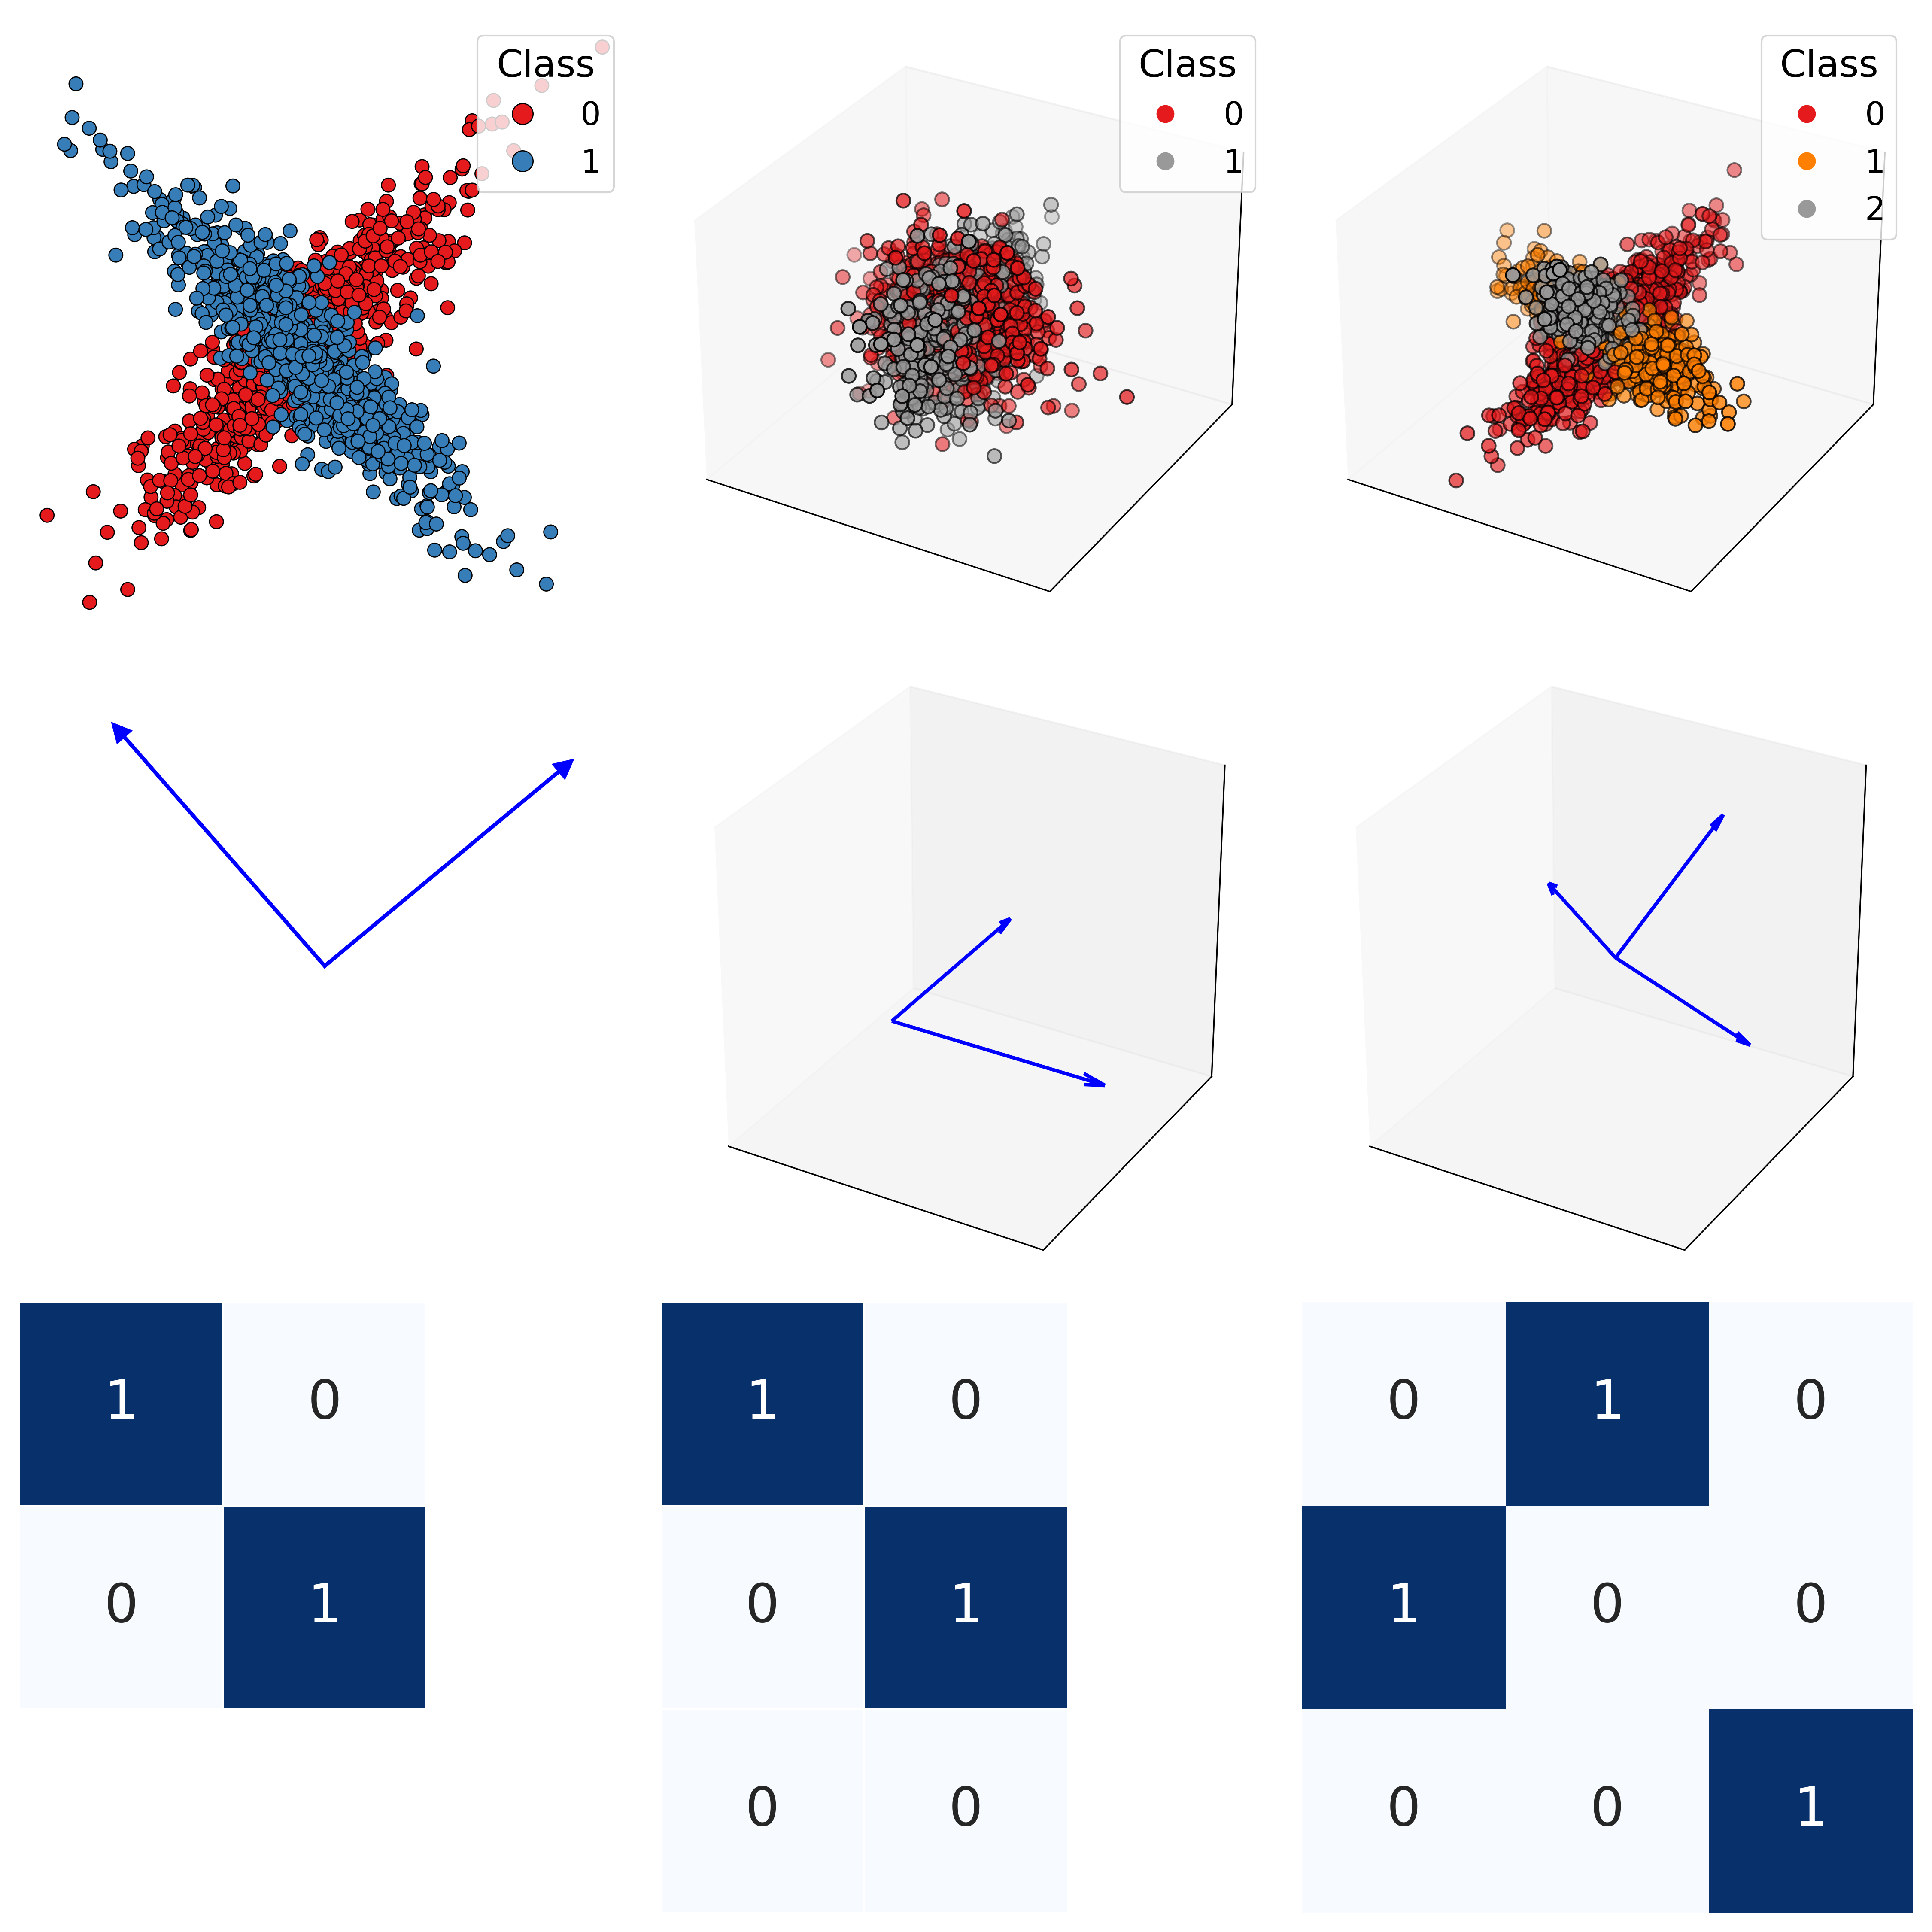
\includegraphics[width=0.4\textwidth]{figs/fig1.png}
    \caption{Visualization of synthetic 2D and 3D datasets (top) and the learned transformation matrix \( e^{A} \) and mapping matrix \( L \) (bottom) using \gls{eca}.}
    \label{fig:combined_visualization}
\end{figure}

\subsection{Sparsity Explanation} \label{sec:explanation} Applying orthogonal transformation $P = e^A$ to input $\mathsf{x}^{(i)}$ yields $\psi^{(i)} = P^\top \mathsf{x}^{(i)}$, where energy concentrates in few components for low-dimensional data~\cite{bandoh2009mathematical, tuqan2000state}.

\subsubsection{Quantum Measurement Analogy} $|\psi_j^{(i)}|^2$ represents eigenfeature $j$'s activation probability for sample $i$, with most values approaching zero for structured data, creating sparsity~\cite{nielsen2010quantum, lin2020sparsity}.

\subsubsection{Role of Mapping Matrix (L)} Matrix $L$ links eigenfeatures to classes while cross-entropy optimization prioritizes high-activation features, inducing sparsity~\cite{lin2020sparsity}.



\section{Results}
We evaluate our method on various datasets, including synthetic 2D and 3D datasets, the Iris dataset~\cite{fisher1936use}, the Digits dataset~\cite{alpaydin1998optical}, MNIST~\cite{lecun1998gradient}, and Fashion MNIST~\cite{xiao2017fashion}. Comparisons are made with \Gls{lor}, \Gls{lda}, \Gls{qda}, \Gls{svm}, and \Gls{ksvm} using the \Gls{rbf} kernel~\cite{hastie2009elements,cortes1995support}. 
\subsection{Synthetic Datasets} 
We assess our model using synthetic datasets with varying degrees of class overlap and non-linear decision boundaries, as shown in Figure~\ref{fig:combined_visualization} (top). Using 2D and 3D datasets, \gls{eca} achieves the highest accuracies of 86.00\% (2D), 74.33\% (3D, two classes), and 73.50\% (3D, three classes), outperforming traditional models. The transformation and mapping matrices (Figure~\ref{fig:combined_visualization}, bottom) illustrate how \gls{eca} captures the underlying data structures.
\subsection{Iris Dataset}
Using the Iris dataset, a standard multiclass classification problem, \gls{eca} achieves a perfect accuracy of 100\%, matching the performance of \Gls{lda}, \Gls{qda}, and \Gls{svm} (Table~\ref{tab: iris}). Figure~\ref{fig:iris_pca_eca} visualizes class separations using \gls{eca} and \Gls{pca}, highlighting the effectiveness of \gls{eca} in enhancing class separation.

\begin{table*}[htbp]
  \centering
  \begin{minipage}[b]{0.23\textwidth}
    \centering
    \caption{Comparison of Classifiers on the Iris Dataset}
    \label{tab: iris}
    \resizebox{\textwidth}{!}{%
    \begin{tabular}{@{}lcc@{}}
        \toprule
        \textbf{Model} & \textbf{Accuracy (\%)} & \textbf{Parameters} \\ \midrule
        \Gls{lor} & 96.67 & 15 \\
        \Gls{lda} & \textbf{100} & 15 \\
        \Gls{qda} & \textbf{100} & 63 \\
        \Gls{svm} & \textbf{100} & 15 \\
        \Gls{ksvm} & 96.67 & 49 \\
        \gls{eca} & \textbf{100} & 26 \\ \bottomrule
    \end{tabular}
    }
  \end{minipage}%
  \hfill
  \begin{minipage}[b]{0.23\textwidth}
    \centering
    \caption{Comparison of Classifiers on the Digits Dataset}
    \label{tab: digits}
        \resizebox{\textwidth}{!}{%
    \begin{tabular}{@{}lcc@{}}
        \toprule
        \textbf{Model} & \textbf{Accuracy (\%)} & \textbf{Parameters} \\ \midrule
        \Gls{lor} & 86.67 & 650 \\
        \Gls{lda} & 95.28 & 650 \\
        \Gls{qda} & 73.33 & 41,610 \\
        \Gls{svm} & 88.06 & 2,925 \\
        \Gls{ksvm} & \textbf{99.17} & 663 \\
        \gls{eca} & \textbf{99.17} & 2,784 \\ \bottomrule
    \end{tabular}
    }
  \end{minipage}%
  \hfill
  \begin{minipage}[b]{0.23\textwidth}
      \centering
    \caption{Comparison on the Fashion MNIST Dataset}
    \label{tab:fashion_mnist}
        \resizebox{\textwidth}{!}{%
    \begin{tabular}{@{}lcc@{}}
        \toprule
        \textbf{Model} & \textbf{Accuracy (\%)} & \textbf{Parameters} \\ \midrule
        \Gls{lor} & 77.14 & 7,850 \\
        \Gls{lda} & 53.57 & 7,850 \\
        \Gls{qda} & 17.86 & 6,154,410 \\
        \Gls{svm} & 77.14 & 35,325 \\
        \Gls{ksvm} & 74.29 & 435 \\
        \gls{eca} & \textbf{80.71} & 316,344 \\ \bottomrule
    \end{tabular}
    }
  \end{minipage}
    \hfill
  % 第四个表格
  \begin{minipage}[b]{0.23\textwidth}
      \centering
    \caption{Comparison on the Downsampled MNIST Dataset}
    \label{tab: mnist}
        \resizebox{\textwidth}{!}{%
    \begin{tabular}{@{}lcc@{}}
        \toprule
        \textbf{Model} & \textbf{Accuracy (\%)} & \textbf{Parameters} \\ \midrule
        \Gls{lor} & 84.29 & 7,850 \\
        \Gls{lda} & 20.71 & 7,850 \\
        \Gls{qda} & 21.43 & 6,154,410 \\
        \Gls{svm} & 85.71 & 35,325 \\
        \Gls{ksvm} & 87.86 & 488 \\
        \gls{eca} & \textbf{88.57} & 316,344 \\ \bottomrule
    \end{tabular}
    }
  \end{minipage}
\end{table*}

\begin{figure*}[ht]
    \centering
    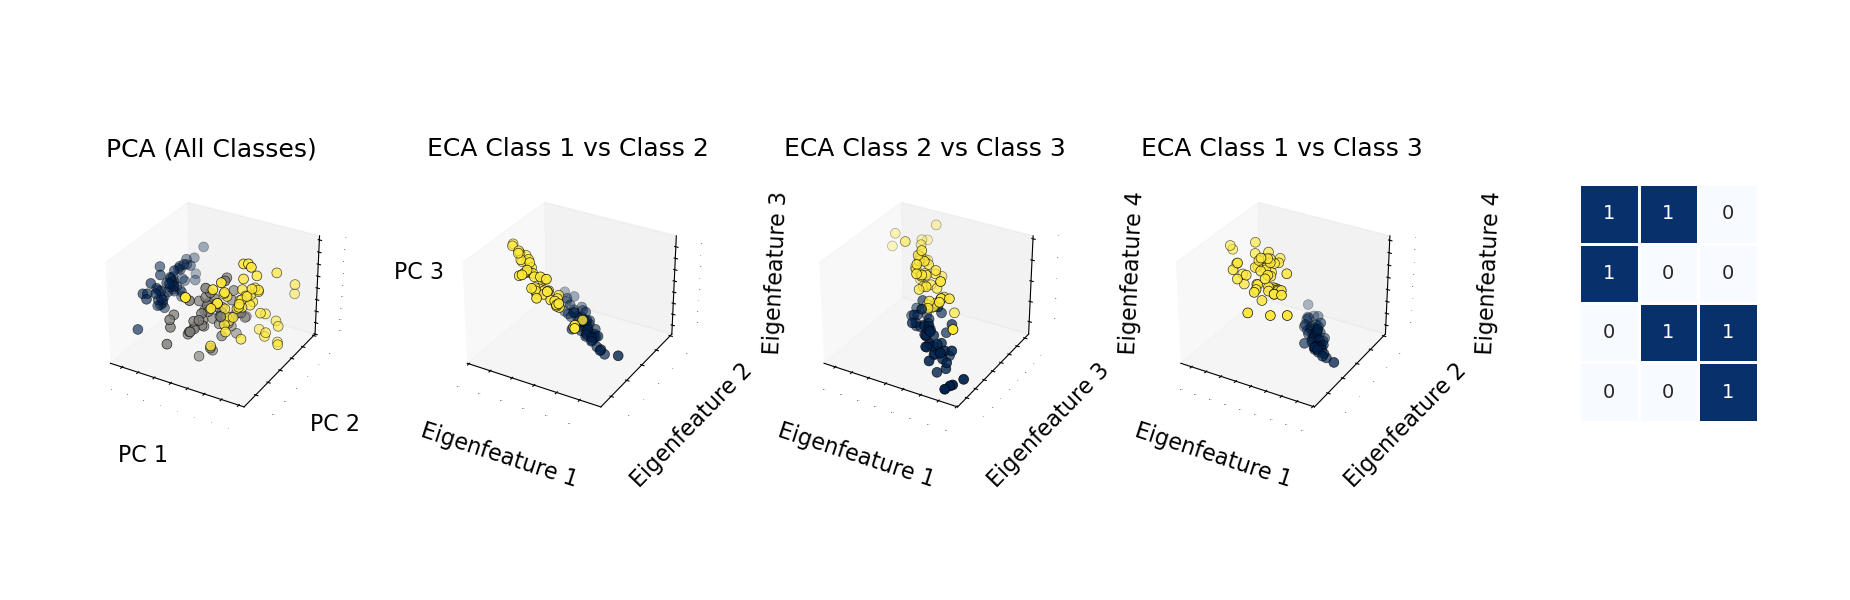
\includegraphics[width=1\linewidth]{figs/fig2.png}
    \vspace{-40pt}
    \caption{
    Comparison of PCA and ECA projections for class separation on the Iris dataset: PCA (left), ECA class 1 vs. 2 (second from left), 2 vs. 3 (third from left), 1 vs. 3 (fourth from left), and L matrix (right)".}
    \label{fig:iris_pca_eca}
\end{figure*}

\begin{figure}[ht]
    \centering
    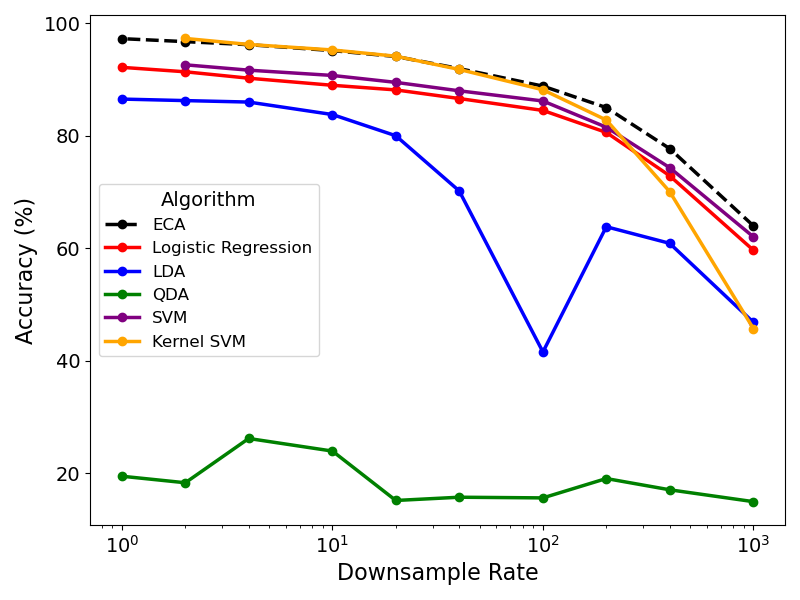
\includegraphics[width=0.9\linewidth]{figs/fig3.png}
    \vspace{-10pt}
    \caption{Accuracy comparison on MNIST varying downsample fractions.}
    \label{fig:mnist_downsample}
\end{figure}

\begin{figure*}[ht]
    \centering
    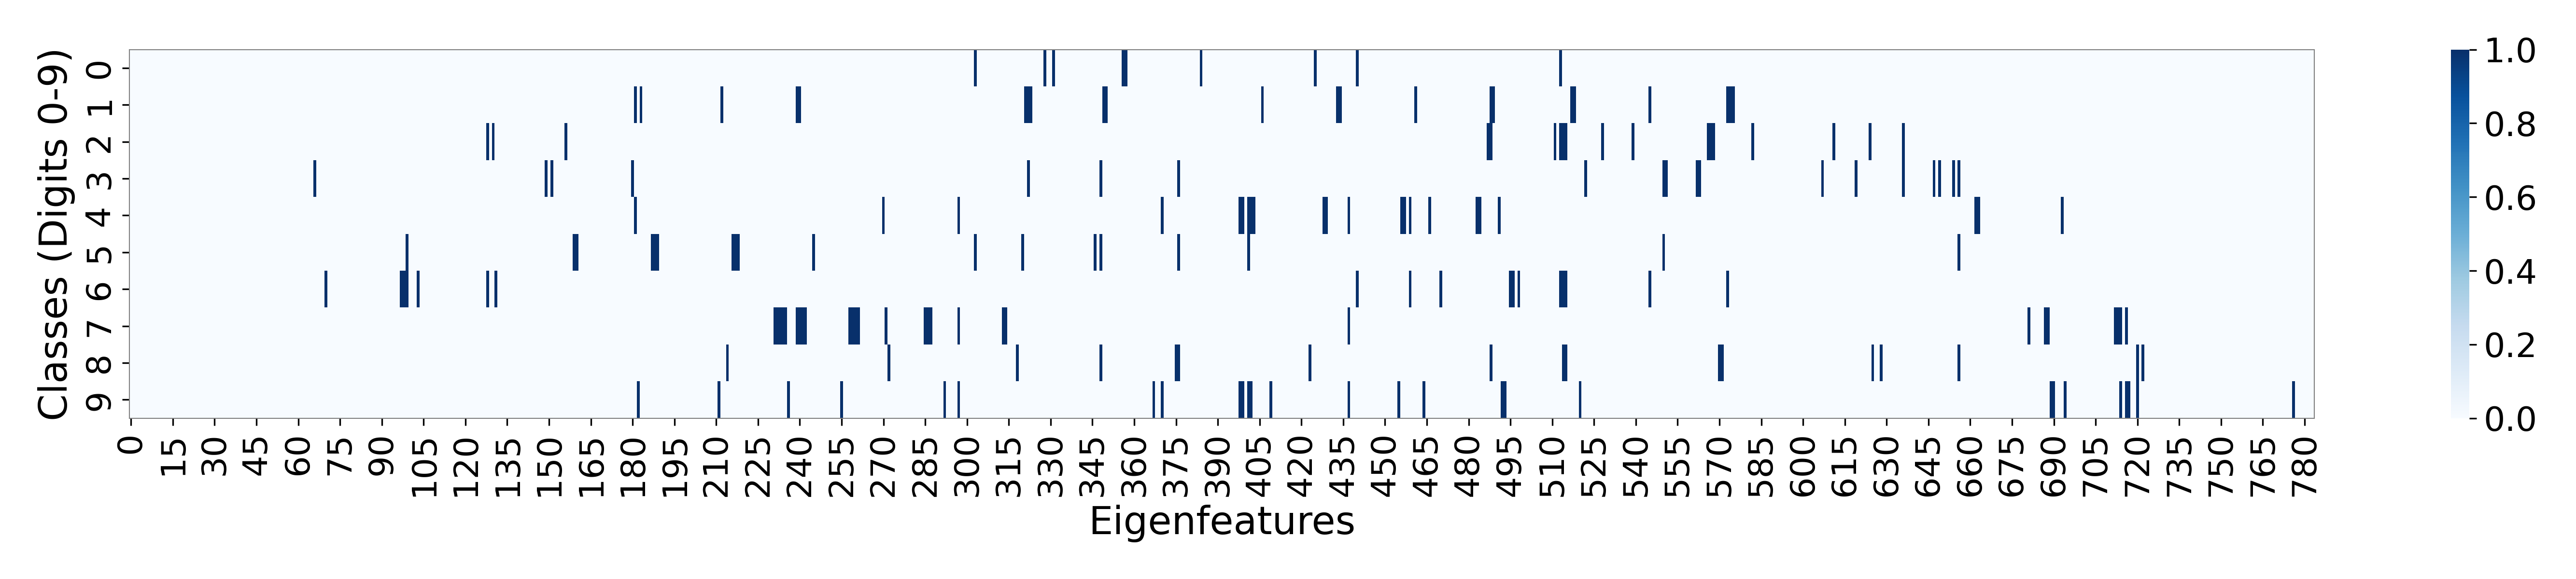
\includegraphics[width=0.95\linewidth]{figs/fig4.png}
    \vspace{-15pt}
    \caption{Heatmap of the mapping matrix $L$ for MNIST: blue intensity indicates eigenfeature-class associations.
    % , highlighting \gls{eca}'s efficient dimensionality reduction and discriminative power.
    }
    \label{fig:mnist_L_heatmap}
\end{figure*}


\subsection{Digits Dataset}
\gls{eca} achieves 99.17\% accuracy on the Digits dataset, equaling \Gls{ksvm} and surpassing other models (Table~\ref{tab: digits}).



\subsection{Fashion MNIST Dataset}
For the Fashion MNIST dataset, Table~\ref{tab:fashion_mnist} indicates that \gls{eca} achieves 80.71\% accuracy, outperforming other linear models while \Gls{qda} struggles due to collinearity issues.
\subsection{MNIST Dataset}
On the downsampled MNIST dataset, \gls{eca} achieves an accuracy of 88.57\%, surpassing \Gls{lor} and closely matching \Gls{svm} (Table~\ref{tab: mnist}). Figure~\ref{fig:mnist_downsample} shows that \gls{eca} consistently outperforms \Gls{lor} and \Gls{lda} across varying sample sizes, demonstrating robustness in sparse data scenarios.

To assess robustness, we vary the training data downsample fraction while keeping the test data ratio fixed at 0.2. Training samples range from 48,000 to 48. As shown in Figure~\ref{fig:mnist_downsample}, \gls{eca} consistently outperforms \Gls{lor} and \Gls{lda}, particularly at lower sample fractions, showing its effectiveness on sparse data.

\begin{figure*}[ht]
    \centering
    \begin{minipage}{0.48\textwidth}
        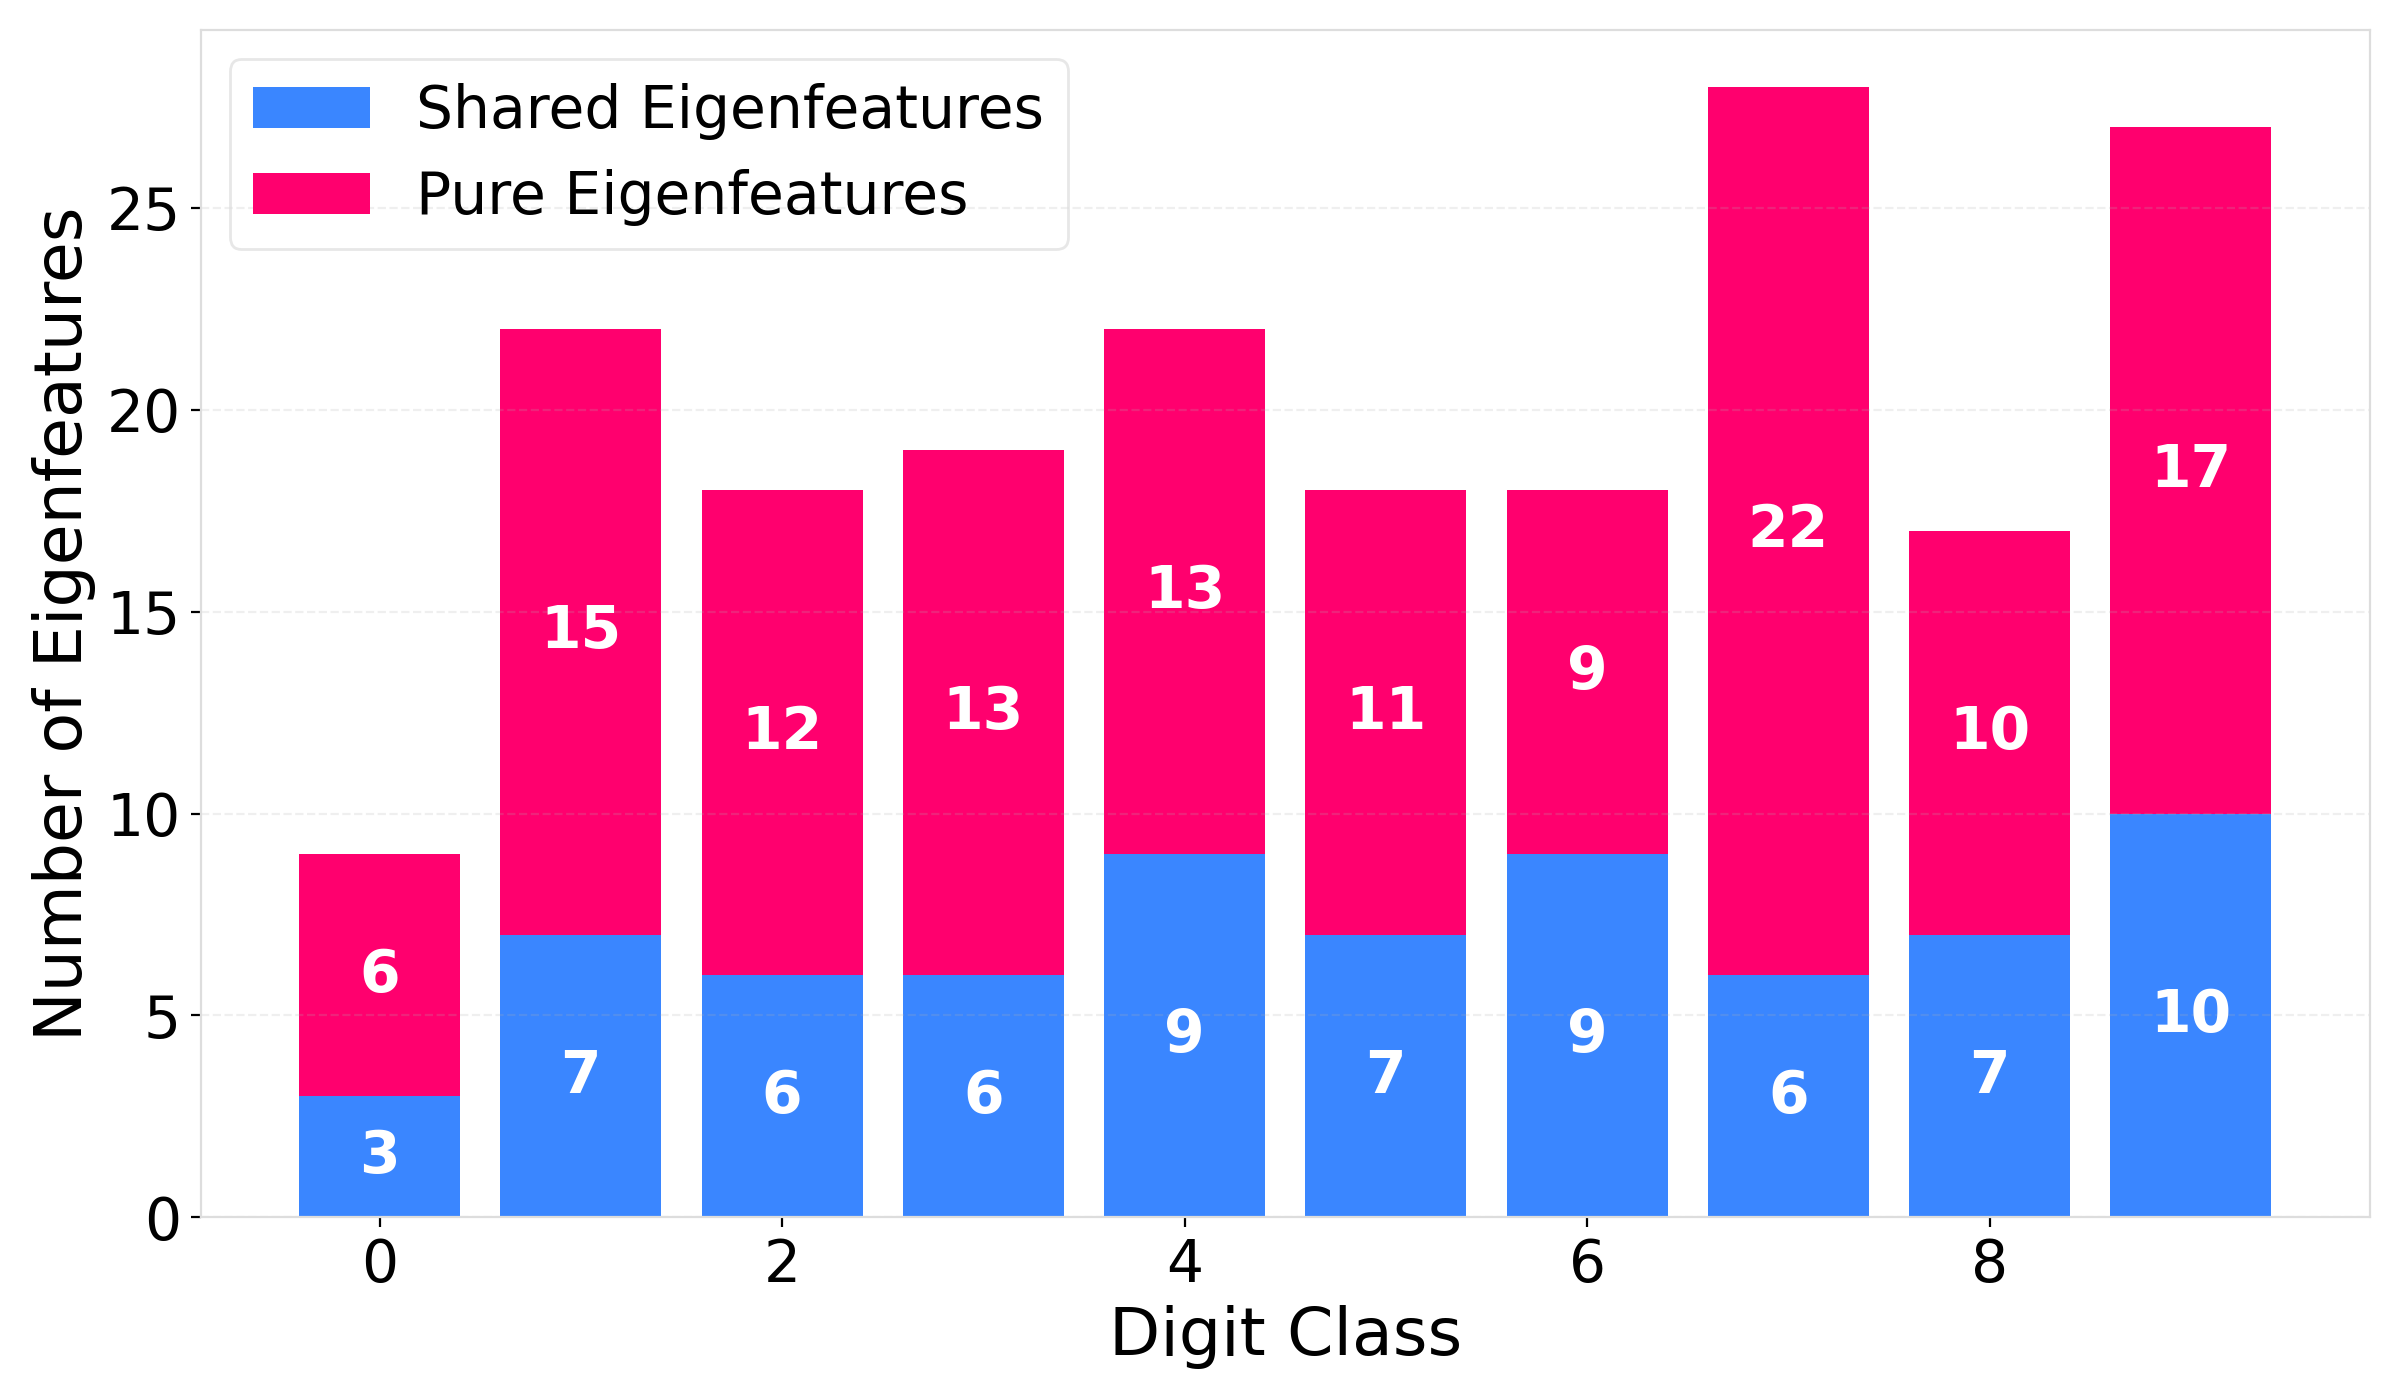
\includegraphics[width=\linewidth]{figs/fig5.png}
        \vspace{-25pt}
        \caption{Distribution of pure and shared eigenfeatures across MNIST classes: pure eigenfeatures (pink) capture class-specific traits, while shared eigenfeatures (blue) represent common patterns, reflecting class complexity.}
        \label{fig:eigenfeature_distribution}
    \end{minipage}
    \hfill
    \begin{minipage}{0.48\textwidth}
        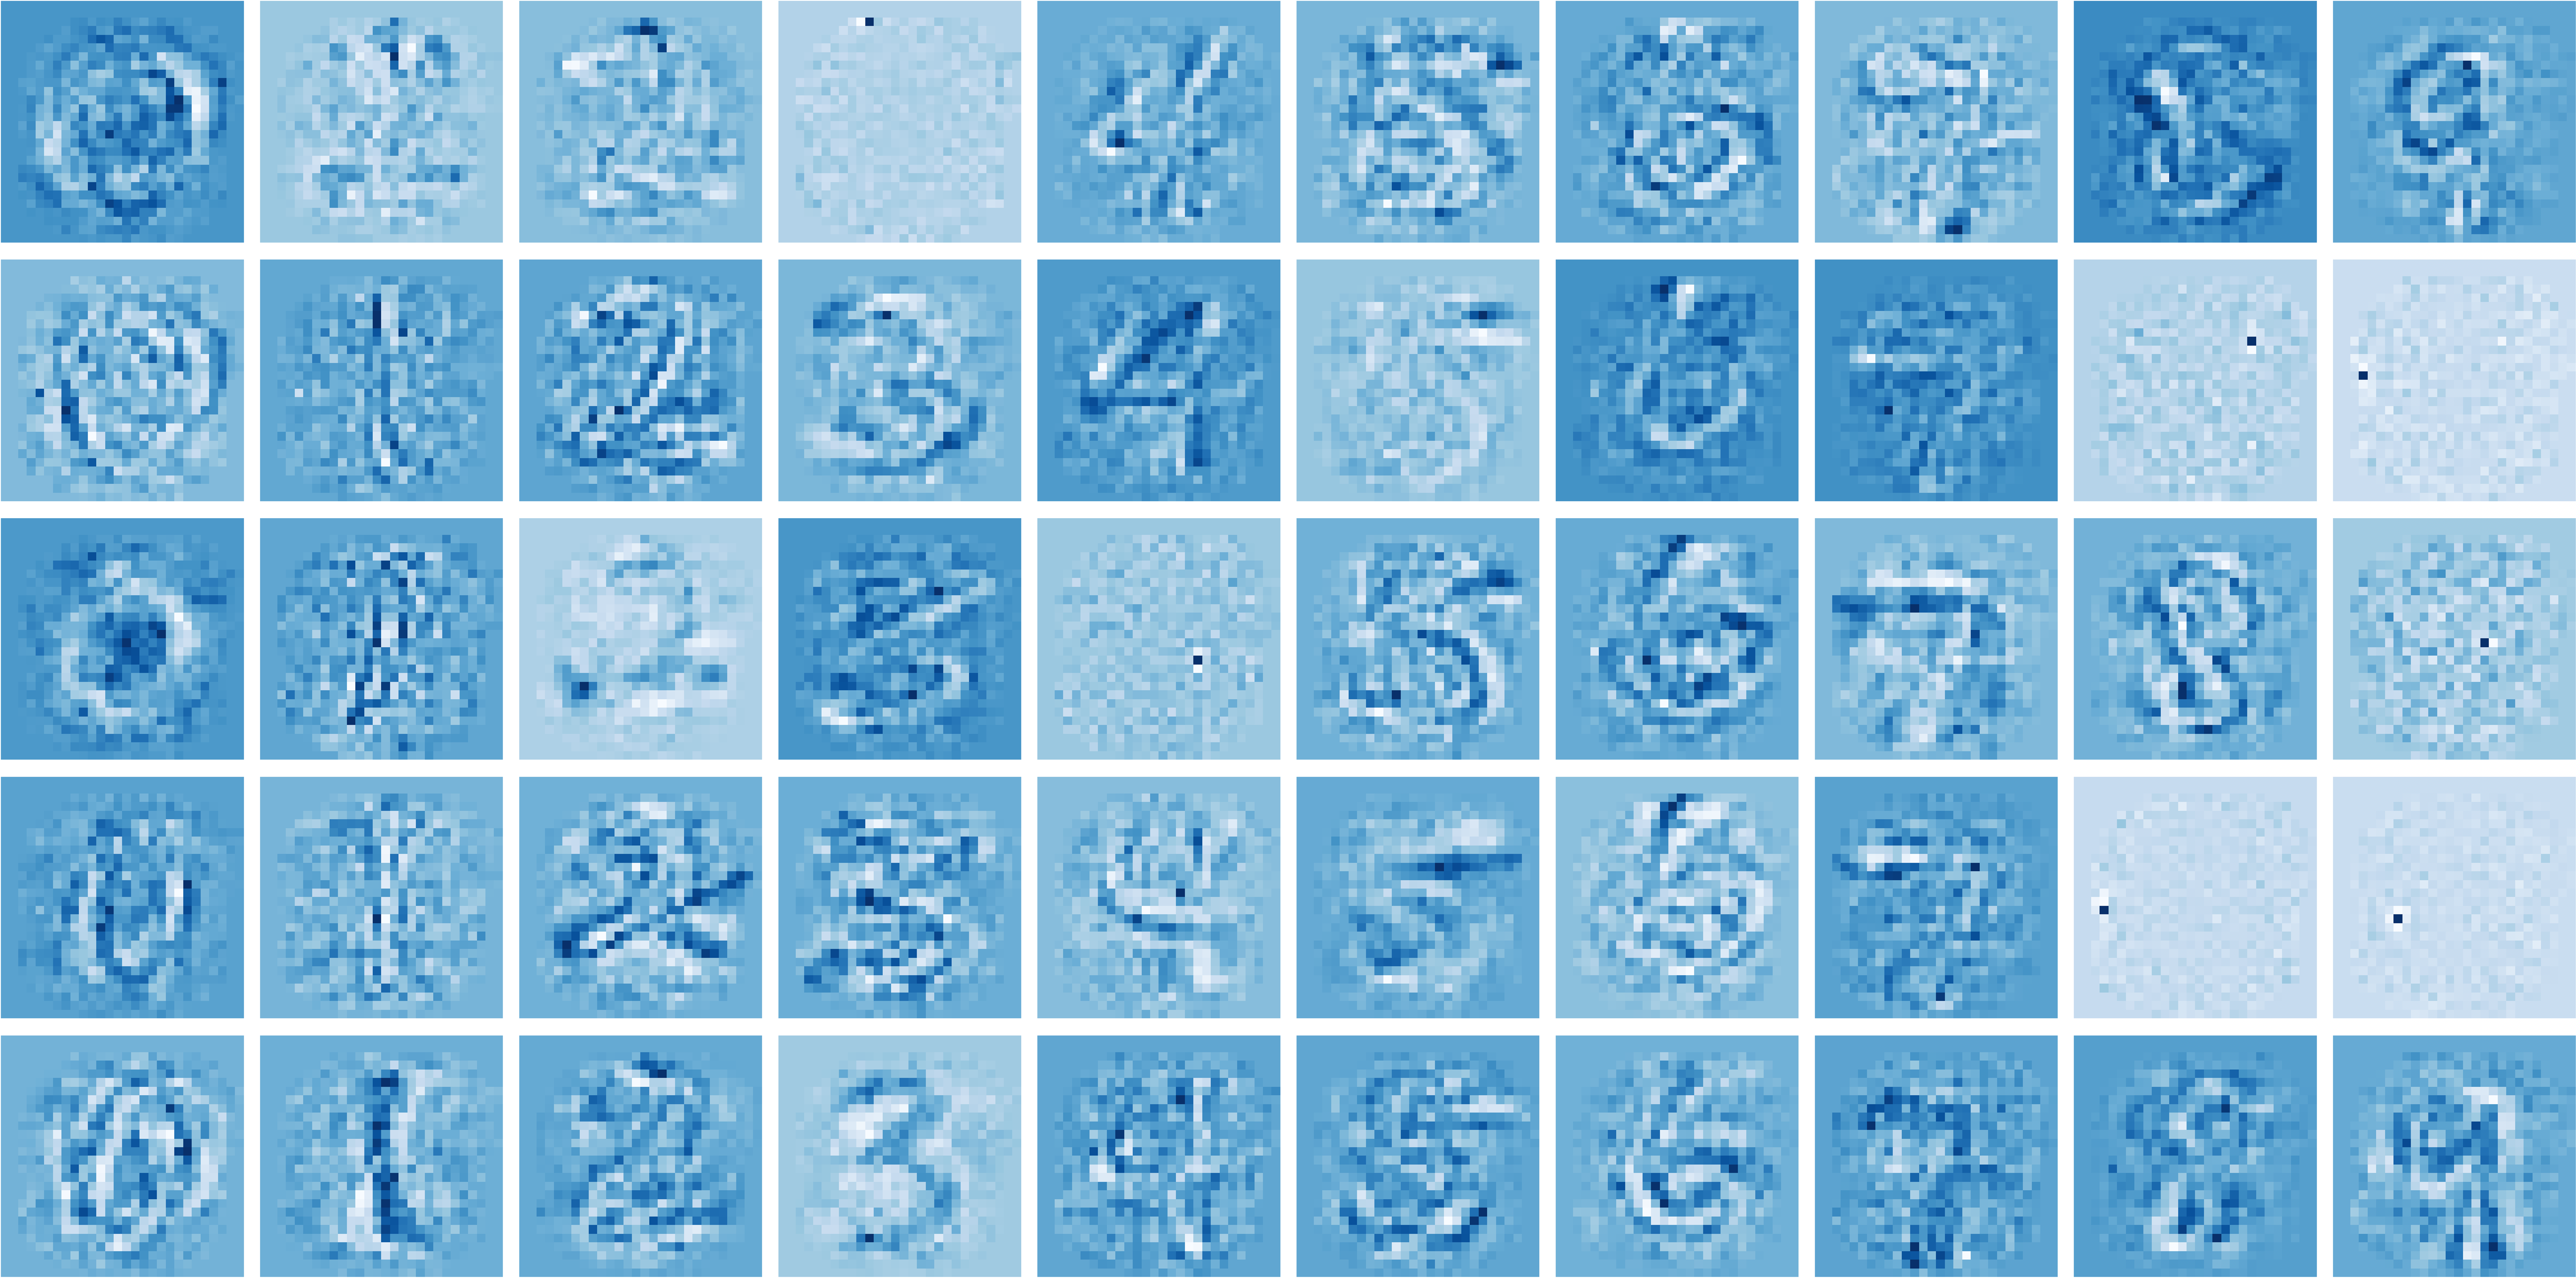
\includegraphics[width=\linewidth]{figs/fig6.png}
        \caption{Visualization of pure eigenfeatures for each MNIST digit class extracted by the \gls{eca} model. Each row shows five representative eigenfeatures capturing class-specific patterns and discriminative characteristics.}
        \label{fig}
    \end{minipage}
\end{figure*}

\begin{figure*}[!htbp]
    \centering
    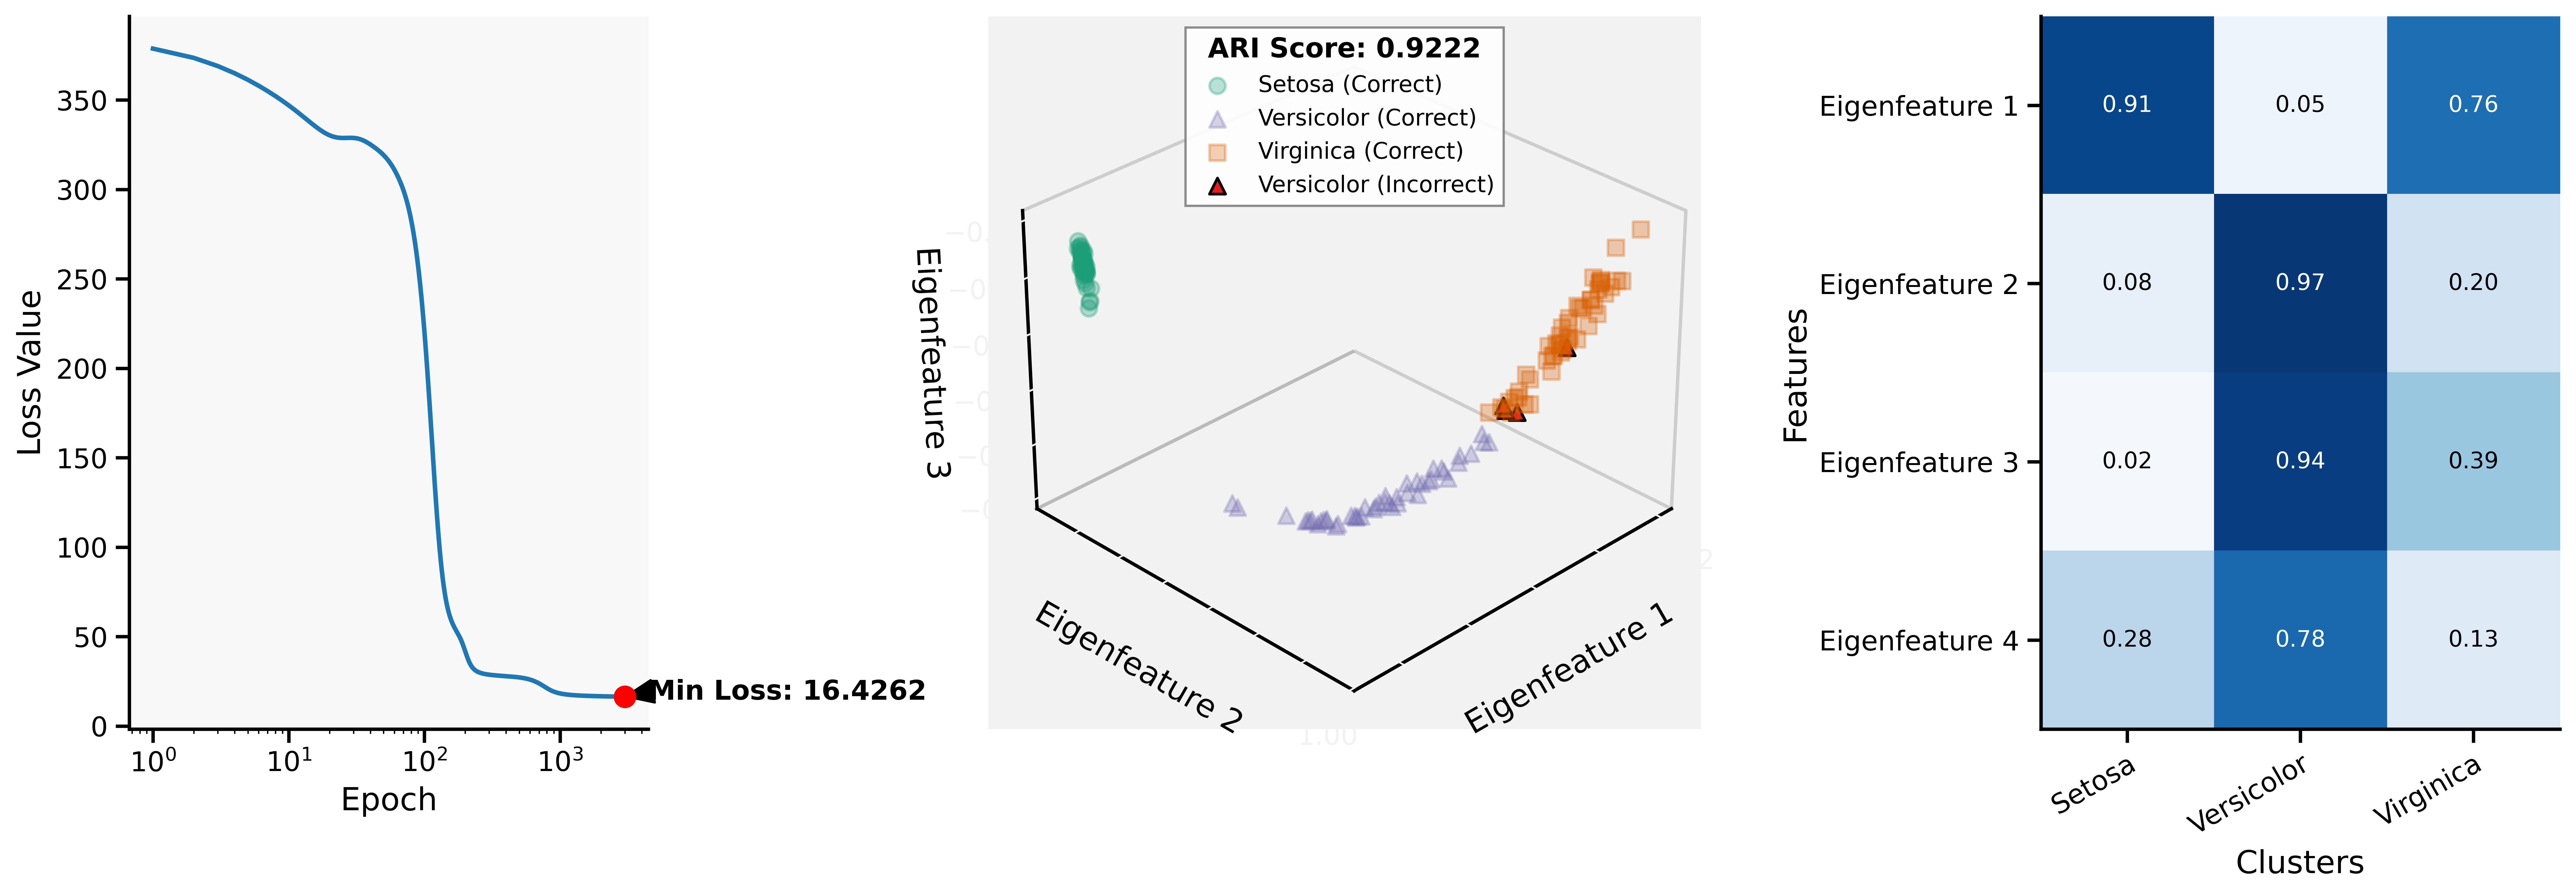
\includegraphics[width=0.925\linewidth,trim={0 0pt 0 0},clip]{figs/fig7.png}
    \vspace{-10pt}
    \caption{Unsupervised ECA on the Iris dataset: training loss curve showing stable convergence around epoch 1500 (left). Data projection onto three principal eigenfeatures, with marker shapes denoting true classes and colors indicating clustering accuracy (middle). L matrix mapping highlighting feature-cluster associations, revealing key features for class separation (right).}
    \label{fig:ueca_iris}
\end{figure*}


\subsection{Eigenfeature Analysis of MNIST}

To evaluate \gls{eca}'s feature extraction ability on high-dimensional images, we analyzed its eigenfeature distribution on MNIST dataset. 
The mapping matrix $L$ (Figure~\ref{fig:mnist_L_heatmap}) highlights the sparse connections between eigenfeatures and digit classes, demonstrating \gls{eca}'s ability to identify a minimal, discriminative subset while maintaining data structure.

Figure~\ref{fig:eigenfeature_distribution} shows pure (class-specific) and shared (multiclass) eigen characteristics. Digit `7' has the most pure eigenfeatures (22), reflecting its structural complexity, while digit `0' has the fewest (9), suggesting simplicity. \gls{eca} achieves a reduction in dimensionality 75\% without reducing discriminative power.

Pure eigenfeatures, visualized in Figure~\ref{fig}, reveal low-dimensional manifold structures leveraged for classification. These vary from digit-like forms to distinctive subcomponents, supporting manifold learning by projecting high-dimensional data onto interpretable, class-specific subspaces. 
As discussed in Section~\ref{sec:explanation}, \gls{eca} naturally yields sparsity without traditional regularization due to:

1) Energy Compaction: 
The orthogonal transformation \(P\) redistributes the input energy such that, if the data lies on a low-dimensional manifold, only a few projection coefficients in \(\psi^{(i)}\) carry significant energy.
2) Quantum Measurement Analogy: Interpreting \( |\psi_j^{(i)}|^2 \) as a probability shows that only a few eigenfeatures are effectively ``observed''.
3) Selective Weighting by \(L\): \(L\) is trained to amplify the contribution of those eigenfeatures with high activation, while features with near-zero activations receive negligible weights.



\subsection{Exploratory Analysis with Unsupervised ECA}

To explore \gls{ueca}'s potential, we applied it to the Iris dataset in an unsupervised context. Figure~\ref{fig:ueca_iris} presents the results, showing the loss convergence (left), data projection onto eigenfeatures with class labels and clustering accuracy (middle), and the $L$ matrix mapping input features to clusters (right). \gls{ueca} achieved an Adjusted Rand Index of $0.92$, indicating strong alignment between clusters and true classes. It effectively separates Setosa from Versicolor and Virginica, managing their overlap.

While we do not position \gls{ueca} as universally superior to established clustering methods,
its orthogonal transformations reveal structural relationships often missed by distance-based approaches.
The resulting eigenfeature projections provide meaningful low-dimensional representations
, underscoring the model's capability to uncover intrinsic data structures.
This suggests promising opportunities for exploring hybrid semi-supervised approaches in future research.

\section{Conclusion}

This paper introduces \gls{eca}, a quantum-inspired model designed to achieve linear separability without requiring data centralization or standardization. \gls{eca} leverages a robust orthogonal transformation to capture intrinsic data structures, enabling effective feature extraction and classification even in distributed and privacy-sensitive environments. Extensive experimentation across various datasets demonstrates that \gls{eca} consistently outperforms traditional linear classifiers,
particularly in complex and resource-constrained settings.

\section*{Acknowledgments}
This work is supported in part by the Research Grants Council (GRF 17201822 and TRS T45-701/22-R) of Hong Kong SAR, China; and in part by Department of Science
and Technology of Guangdong Province (2023B0909020003).

\bibliographystyle{IEEEtran}
\bibliography{ref}
\vfill

\end{document}


